\subsection{O teorema}

Exploraremos os caminhos não cruzantes providos por processos de Markov. Considere uma partícula de movendo com uma regra qualquer, vamos descrever esse movimento de forma que denotaremos $p_t(a;x)$ a densidade de probabilidade de transição; isto é, a chance uma partícula em $a$ ir para $x$ em um próximo momento. Um teorema clássico enuncia a probabilidade de um certo número de caminhos não se intersectarem passado um tempo $t$.

O teorema diz: Considere $X_1(t), \dots, X_n(t)$ cópias independentes de um processo forte de Markov com caminhos condicionados tais que

\[
	X_j(0) = a_j
\] 

onde \cmany{a}{n}{<} são valores dados. Notamos novamente $p_t(x, y)$ ser a densidade do processo de transição. Vamos definir regiões \many{E}{n} onde $E$'s vizinhos não se intersectam. Temos

\[
	\int_{E_1} \dots \int_{E_n} \det{[p_t(a_i, x_j)]^{n}_{i,j=1}} dx_1 \dots dx_n
\]

vai ser a probabilidade de que os caminhos não tenham se intersectados no intervalo de tempo $[0, t]$ e $X_j(t)$ nos intervalos correspondentes. A demonstração está em \cite{ArnoLectureNotes}. Note que temos

\[
\int_{E_1} \dots \int_{E_n} \det{[p_t(a_i, x_j)]^{n}_{i,j=1}}  dx_1 \dots dx_n
\]

\begin{align}
	& = \int_{E_1} \dots \int_{E_n}
	\begin{vmatrix}
		p_t(a_1, x_1) 	& p_t(a_2, x_1) 	 & \dots	& p_t(a_{n-1}, x_1) 	& p_t(a_n, x_1) \\
		p_t(a_1, x_2) 	& p_t(a_2, x_2) 	 & \dots 	&  p_t(a_{n-1}, x_2)				&  p_t(a_n, x_2) \\
		\vdots 			& \vdots 			 & \vdots 	& \vdots 				& \vdots \\
		p_t(a_1, x_{n-1}) & p_t(a_2, x_{n-1})& \dots 	&  	p_t(a_{n-1}, x_{n-1})	& p_t(a_n, x_{n-1}) \\
		p_t(a_1, x_n) 	& p_t(a_2, x_n) 	 & \dots  	& p_t(a_{n-1}, x_n) 	& p_t(a_n, x_n)
	\end{vmatrix} dx_1 \dots dx_n \\ 
	& = \sum_{\sigma}sgn(\sigma) \prod_{j=1}^{n} p_t(a_j, E_{\sigma(j)}) \\
	& = \sum_{\sigma} sgn(\sigma) \mathcal{P}(A_\sigma)
	\label{eq: detInd}
\end{align}

Onde denotamos

\[
	p_t(a_j, E_{\sigma(j)}) = \int_{E_j} p_t(a_i, x_j) dx_j
\]

$\sigma$ é uma permutação de ${1, \dots, n}$ e $A_{\sigma}$ é o evento que $X_j(t) \in E_{\sigma(j)}$ para todo $j$. Os caminhos devem ser independentes para \eqref{eq: detInd}.

De alguma forma o determinada permuta os caminhos em todas ordens possíveis e calcula a probabilidade de todos se manterem nos intervalos adequados. Um exemplo de baixas dimensões pode mostrar que


\begin{align}
	&
	\begin{vmatrix}
		p_t(a_1, x_1) & p_t(a_2, x_1) & p_t(a_3, x_1) \\
		p_t(a_1, x_2) & p_t(a_2, x_2) & p_t(a_3, x_2) \\
		p_t(a_1, x_3) & p_t(a_2, x_3) & p_t(a_3, x_3)
	\end{vmatrix} =\\
	&
	+ p_t(a_1, x_1) p_t(a_2, x_2) p_t(a_3, x_3)  \\
	&
	+ p_t(a_2, x_1) p_t(a_3, x_2) p_t(a_1, x_3) \\
	&
	+ p_t(a_3, x_1) p_t(a_1, x_2) p_t(a_2, x_3) \\
	& 
	- p_t(a_3, x_1) p_t(a_2, x_2) p_t(a_1, x_3) \\
	&
	-  p_t(a_2, x_1) p_t(a_1, x_2) p_t(a_3, x_3) \\
	&
	- p_t(a_1, x_1) p_t(a_3, x_2) p_t(a_2, x_3)
\end{align}

Logo

\begin{align}
	\int_{E_1} \dots \int_{E_n} \det{[p_t(a_i, x_j)]^{n}_{i,j=1}}  dx_1 \dots dx_n  = 
	&
	+ p_t(a_1, E_1) p_t(a_2, E_2) p_t(a_3, E_3)  \\
	&
	+ p_t(a_2, E_1) p_t(a_3, E_2) p_t(a_1, E_3) \\
	&
	+ p_t(a_3, E_1) p_t(a_1, E_2) p_t(a_2, E_3) \\
	& 
	- p_t(a_3, E_1) p_t(a_2, E_2) p_t(a_1, E_3) \\
	&
	-  p_t(a_2, E_1) p_t(a_1, E_2) p_t(a_3, E_3) \\
	&
	- p_t(a_1, E_1) p_t(a_3, E_2) p_t(a_2, E_3)
\end{align}

Onde somamos os casos onde as partículas se matém ordenadas e subtraímos os casos onde elas se cruzam.


\subsection{Consequências}

Considere $n$ cópias do processo de Markov condicionado para começar em $t=0$ nas determinadas posições \cmany{a}{n}{<}. Se condicionarmos estes processos para não intersectar no intervalo $[0,t]$, o teorema vai nos dizer que os caminhos em um tempo $t$ vão ter uma densidade de probabilidade conjunta

\[
	\frac{1}{\mathcal{Z}_n} \det{[p_t(a_i, x_j)]^{n}_{i,j=1}}
\]

Mas este não pode ser considerado um processo pontual determinado. Não é expresso por um produto de determinantes. Isso pode ser ajeitado se considerarmos um tempo $T > t$ no nosso processo. Tomaremos \many{b}{n} posições finais e condicionaremos os caminhos a não intersectar no intervalo $[0, T]$ com $X_j(0) = a_j$ e $X_j(T) = b_j$ para todos. É possível mostrar que a distribuição conjunta deles será

\[
	\frac{1}{\mathcal{Z}_n'} \det{[p_t(a_i, x_j)]^{n}_{i,j=1}} \det{[p_{T-t}(x_i, b_j)]^{n}_{i,j=1}}
\]

Que será biortogonal com as funções

\[
	f_j = p_t(a_j, x) \ ; \ g_j = p_{T-t}(x, b_j)
\]

E nosso caso de interesse é quando $a_j \rightarrow a$ e $b_j \rightarrow b$. Note que usando as duas funções podemos forçar que o movimento browniano se inicie em um ponto e encerre em outro determinado. Em uma, reverteremos o tempo e, nos limites $0$ e $T$, forçaremos que apenas uma das funções seja predominante de forma que a posição inicial de cada uma prevaleça. Podemos impor a posição inicial e final do movimento. No caso browniano teremos

\[
	p_t(a, x) = \frac{1}{\sqrt{2\pi t}} e^{-\frac{(x-a)^2}{2t}}
\]

No caso dos limites de $a_i \rightarrow a$ e $b_j \rightarrow b$ ficamos, por consequência que quando mais de um $a_i$ ou $b_j$ convergem ao mesmo ponto teremos $\mathcal{Z} \rightarrow 0$ pela sua dependência destes termos (eles não serão mais 'ortogonais', pontos distintos). Por exemplo, para o limite

\[
	\lim_{a_n \rightarrow a_{n-1}} \frac{\det{[p_t(a_i, x_j)]^{n}_{i,j=1}} \det{[p_{T-t}(x_i, b_j)]^{n}_{i,j=1}}}{\mathcal{Z}_n'}
\]


Queremos aplicar L'Hôpital para resolver a indeterminação. Para o determinante podemos notar que

\begin{align*}
	\frac{\partial}{\partial a_n}
	\begin{vmatrix}
		p_t(a_1, x_1) & \dots & p_t(a_1, x_n) \\
		\vdots &\ddots & \vdots \\
		p_t(a_n, x_1) & \dots & p_t(a_n, x_n)
	\end{vmatrix} =
	& 	\frac{\partial}{\partial a_n} [
	p_t(a_n, x_1)
	\begin{vmatrix}
		\dots
	\end{vmatrix}
	 + \dots +
	 p_t(a_n, x_n)
	 \begin{vmatrix}
	 	\dots
	 \end{vmatrix}
	] \\
	& [
	\frac{\partial}{\partial a_n} p_t(a_n, x_1)
	\begin{vmatrix}
		\dots
	\end{vmatrix}
	+ \dots +
	\frac{\partial}{\partial a_n} p_t(a_n, x_n)
	\begin{vmatrix}
		\dots
	\end{vmatrix}
	] \\
	& = \begin{vmatrix}
		p_t(a_1, x_1) & \dots & p_t(a_1, x_n) \\
		\vdots &\ddots & \vdots \\
		\frac{\partial}{\partial a_n} p_t(a_n, x_1) & \dots & \frac{\partial}{\partial a_n} p_t(a_n, x_n)
	\end{vmatrix}
\end{align*}

No limite que estamos tratando:

\[
\begin{vmatrix}
	p_t(a_1, x_1) & \dots & p_t(a_1, x_n) \\
	\vdots &\ddots & \vdots \\
	\frac{\partial}{\partial a_{n-1}} p_t(a_{n-1}, x_1) & \dots & \frac{\partial}{\partial a_{n-1}} p_t(a_{n-1}, x_n)
\end{vmatrix}
\]

Para que todos $a_i \rightarrow a$ precisamos ainda fazer $a_{n-1} \rightarrow a_{n-2}$, $a_{n-2} \rightarrow a_{n-3}$ e assim por diante. Se fizermos assim, terminaremos com

\[
	det\left[ \frac{\partial^{i-1}}{\partial a^{i-1}} p_t(a_i, x_j) \right]_{i,j=1}^{n} 
\] 

Onde

\[
	\frac{\partial^{i-1}}{\partial a^{i-1}} p_t(a_i,x_j) = \left[ \left( \frac{x_j - a_i}{t} \right)^{i-1} + O\left( \frac{x_j - a_i}{t} \right)^{i-2} \right] p_t(a_i,x_j)
\]

Que nos permite afirmar que o determinante é proporcional à

\[
	\det{[x_{j}^{i-1}]}^{n}_{i,j=1} \prod_{j=1}^{n} e^{-\frac{x_j^2 - 2ax_j}{2t}}
\]

quando $a_i \rightarrow 0$. Analogamente para o outro determinante

\[
	\det{[x_{j}^{i-1}]}^{n}_{i,j=1} \prod_{j=1}^{n} e^{-\frac{x_j^2 - 2bx_j}{2(T-t)}}
\]

Ou seja;

\[
	f_j = F_{j-1}(x)e^{-\frac{(x-a)^2}{2t}} \ ; \ g_j = G_{j-1}(x)e^{-\frac{(x-b)^2}{2(T-t)}}
\]

onde $F$ e $G$ são polinômios em $x$  de grau $j-1$. Tomaremos agora o limite em que $a,b \rightarrow 0$. Reescrevemos a distribuição conjunta destes pontos

\begin{align}
	P(x_1, \dots, x_n)
	& = \frac{1}{\mathcal{Z}_n} \det{[p_t(a_i, x_j)]^{n}_{i,j=1}} \det{[p_{T-t}(x_i, b_j)]^{n}_{i,j=1}} \\
	& = \frac{1}{\mathcal{Z}_n} \det{[x_{j}^{i-1}]}^{n}_{i,j=1} \prod_{j=1}^{n} e^{-\frac{x_j^2}{2t}} \det{[x_{j}^{i-1}]}^{n}_{i,j=1} \prod_{j=1}^{n} e^{-\frac{x_j^2}{2(T-t)}} \\
	& =\frac{1}{\mathcal{Z}_n} \det{[x_{j}^{i-1}]}^{n}_{i,j=1} \det{[x_{j}^{i-1}]}^{n}_{i,j=1} \prod_{j=1}^{n} e^{-\frac{T x_j^2}{2t(T-t)}}
\end{align}

Onde o último passo é dado pelo valor do determinante de Vandermonde discutido no apêndice \ref{apdx: vandermonde} tal que

\[
	P(x_1, \dots, x_n)=\frac{1}{\mathcal{Z}_n} \prod_{1\leq i < j \leq n} (x_j - x_i)^2 \prod_{j=1}^{n} e^{-\frac{T x_j^2}{2t(T-t)}}
\] 

Relembrando a equação \eqref{eq: weyl}, podemos interpretar esta distribuição como uma distribuição de autovalores em um espaço de matrizes hermitianas do GUE com entradas de variância $\sigma^2 = \frac{2t(T-t)}{T}$ e média $\mu = 0$. De forma que poderemos simular a evolução destes movimentos brownianos com o sistema de matrizes descrito.

\begin{center}
	\begin{tikzpicture}
		\begin{axis}[
			enlargelimits=true,
			width=0.8\textwidth,
			title={Dyson Bridge},
			legend pos=north west,
			ymajorgrids=true,
			xmajorgrids=true,
			grid style=dashed,
			yticklabel pos=left,
			xlabel={Time},
			ylabel={Y},
			]
			
			\foreach \p in {0,...,19} {
					\addplot+[solid,mark=none]
					table [col sep=comma]
					{data/brownian/b\p};	
			}
			
		\end{axis}
	\end{tikzpicture}
\end{center} 

\inputminted[
frame=lines,
framesep=2mm,
baselinestretch=1.2,
bgcolor=white,
fontsize=\footnotesize,
linenos
]{Python}{code/DysonBridge.py}

Uma outra pergunta sem resposta para mim é: Como simular sistemas com dois pontos finais? Nesse caso pudemos retirar matrizes com entradas independentes porquê a distribuição era relacionada à $e^{\alpha H^2}$, mas agora teremos algo do tipo $e^{\alpha H^2 + H_0}$. Como fazer isso? Podemos tomar duas abordagens temporárias.

\begin{enumerate}
	\item Múltiplos movimentos independentes com finais distintos ordenando os autovalores para participar de cada um dos grupos.
	
	\inputminted[
	frame=lines,
	framesep=2mm,
	baselinestretch=1.2,
	bgcolor=white,
	fontsize=\footnotesize,
	linenos
	]{Python}{code/BrownianMultFinalOpt1.py}
	
	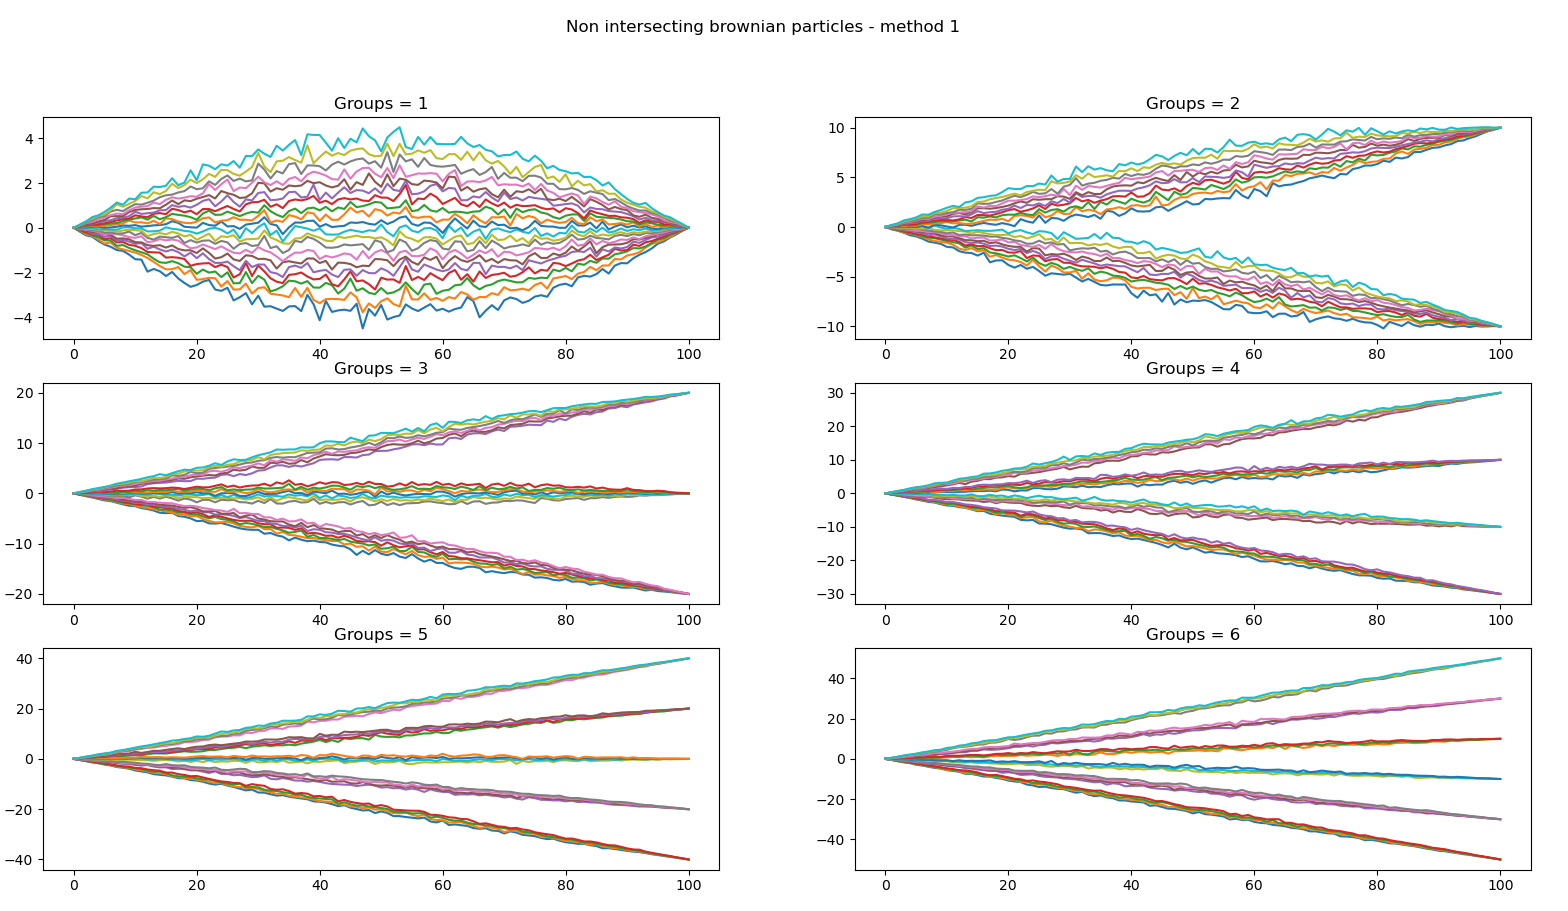
\includegraphics[width=\textwidth]{nonintersectBrownianPart-M1}


	\item Múltiplos movimentos selecionando simulações onde os autovalores não se intersectem.
	
	\inputminted[
	frame=lines,
	framesep=2mm,
	baselinestretch=1.2,
	bgcolor=white,
	fontsize=\footnotesize,
	linenos
	]{Python}{code/BrownianMultFinalOpt2.py} 
	
	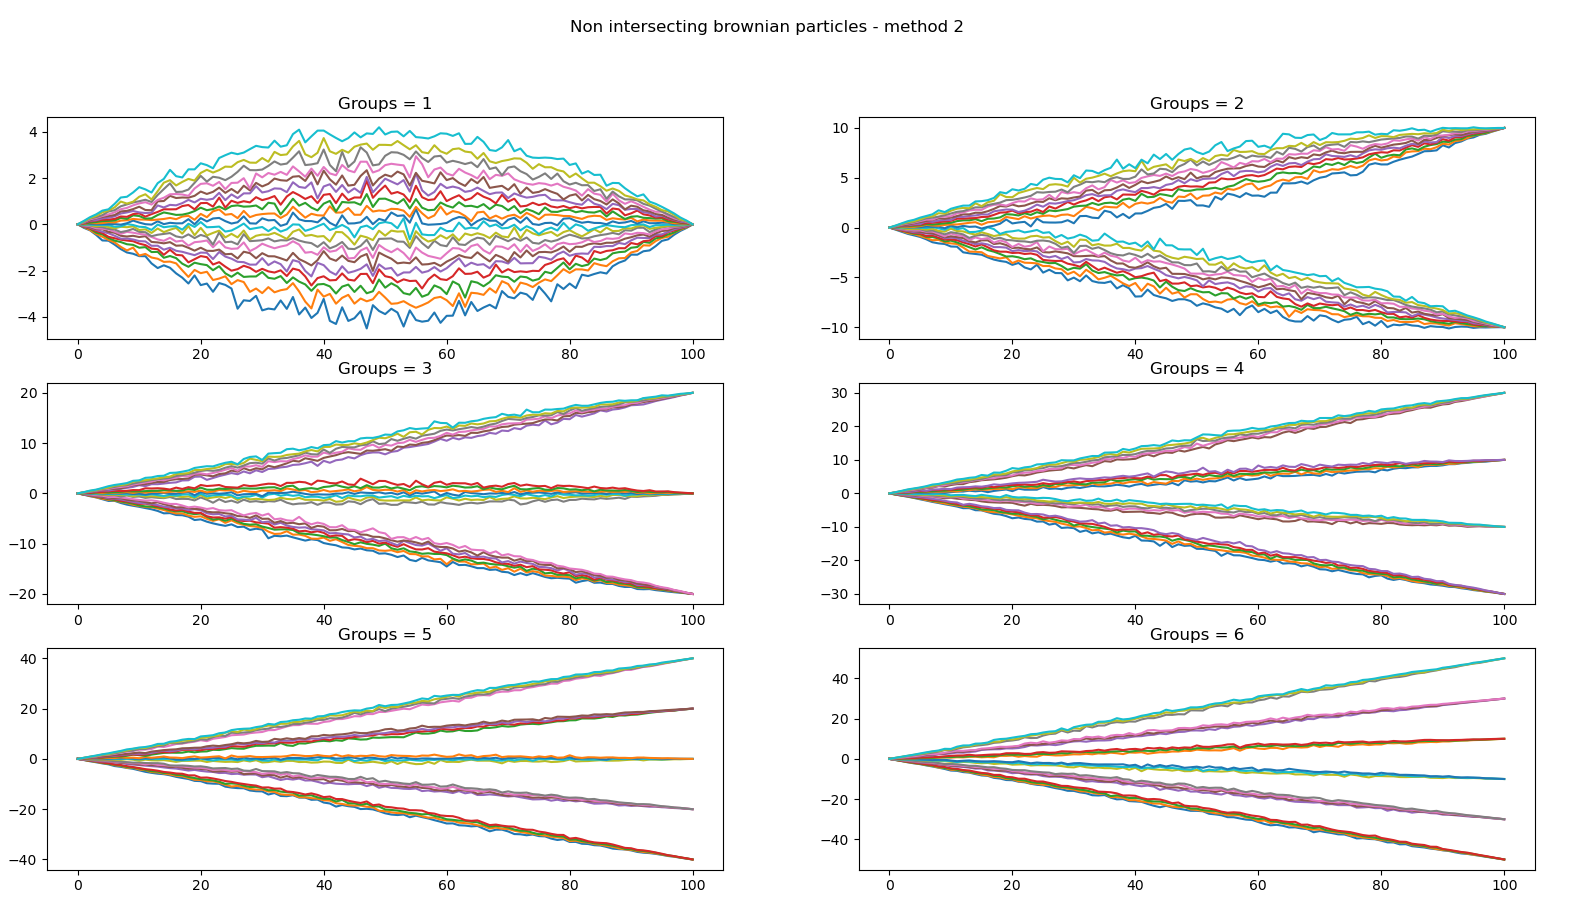
\includegraphics[width=\textwidth]{nonintersectBrownianPart-M2}
	
	
\end{enumerate}

Por fim, podemos mostrar o formato geral destes modelos que tratamos acima.

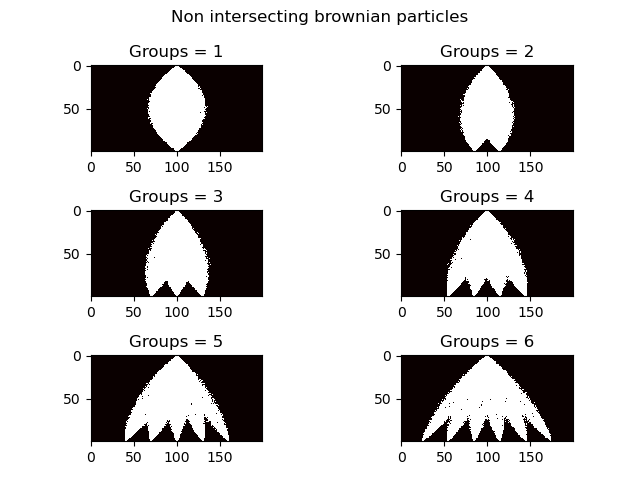
\includegraphics[width=\textwidth]{nonintersectBrownianPart}





